Conformability analysis determines fusible statements of a HorseIR program for code
generation. Using the output of shape analysis, we partition the data dependence graph
into \textit{fusible sections} and the remaining independent statements. Two statements
are in the same fusible section if they are conformable.

\subsection{Fusible Sections}

A fusible section is a subgraph of the program data dependence graph. Let $G=(V, E)$
represents the data dependence graph with statement nodes and dependence edges. Note
that for each statement there is one incoming edge per parameter. The complete graph
$G$ can be divided into two parts: fusible ($\Gamma_F$) and non-fusible ($\Gamma_N$)
disjoint subgraphs.

\subsection{Conformability}

Two statements are conformable if they may be fused in the generated code, thereby
eliminating intermediate results. As with the shape analysis, this check is conservative,
fusing statements only if provably correct. Trivially, element-wise functions operating on
the same vector shape may be fused, but we can also fuse both boolean selection and
reductions. The basic rules for conformability are described in \refTable{tab:conformability}.
\begin{table}[htbp]
\centering
\caption{Conformable rules for two shapes} \label{tab:conformability}
\begin{small}
\begin{tabular}{c||c|c|c|c}
\hline
      & \shapeS  & \shapeV{$c_0$} & \shapeV{$d_0$} & \shapeVS{$a_0$} \\ \hline
\hline
\shapeS & \pass & \notok  & \notok & \notok  \\ \hline
\shapeV{$c_1$} & \notok & $c_0$==$c_1$ & \notok & cond($a_0$,$c_1$) \\ \hline
\shapeV{$d_1$} & \notok & \notok & $d_0$==$d_1$ & cond($a_0$,$d_1$) \\ \hline
\shapeVS{$a_1$}& \notok & cond($a_1$,$c_0$) & cond($a_1$,$d_0$) & $a_0$==$a_1$ \\ \hline
\multicolumn{5}{c}{cond(a,y) is \pass if a.size == y else \notok } \\
\hline
\end{tabular}
\end{small}
\end{table}
In our approach, we check conformability between statements and their
\textit{definition statements} of the input parameters (predecessors in the data
dependence graph).

\subsubsection{Algorithm}

Conformability analysis produces a list of fusible sections given the conformability of
the statements. It traverses bottom up on the dependency graph (reverse topological order),
and recursively fuses definition statements that are conformable with their uses. Each
recursive call tree therefore forms a single fused section that ends when no more
statements may be fused. In addition to conformability, we ensure that reductions may
only terminate fused sections and not be internal nodes. This restriction is due to the
synchronization and implicit data-dependence introduced by the reduction behaviour.
Our algorithm for vector fusion is described in detail in \refAlgo{algo:conformability}
and subsequent sections.

\begin{algorithm}[htbp]
\begin{small}
\SetAlgoLined
\KwIn{Data dependence graph G}
\KwOut{A list of fusible sections}
let $\varnothing$ be an empty vector\;
allStmts $\gets$ reversed topological order of the graph G\;
\ForEach{stmt A in allStmts}{
    \If{ isNotVisited(A) } {
        \uIf{getOp(A) is a reduction function}{ 
            section $\gets$ findFromReduction(A)\;
        } 
        \Else{
            section $\gets$ findFusibleSection(A)\;
        }
    }
}
\SetKwFunction{Funca}{findFusibleSection}
\SetKwProg{Fna}{Function}{:}{}
\Fna{\Funca{A}}{
    \uIf{isNotVisited(A)}{
        setVisited(A)\;
        % \If{isOpInGroupWithoutR(A)}{
        \uIf{isGroupE_Binary(A) or isGroupS(A)}{
            list $\gets$ fetchFusibleStmts(A, A.first.parent)\;
            list.append(fetchFusibleStmts(A, A.second.parent))\;
        }
        \uElseIf{isGroupE_Unary(A) or isGroupB(A)}{
            list $\gets$ fetchFusibleStmts(A, A.first.parent)\;
        }
        \uElseIf{isGroupX(A)}{
            list $\gets$ fetchFusibleStmts(A, A.second.parent)\;
        }
        \Else{
            list $\gets$ $\varnothing$\;
        }
        \Return{\{A\}.append(list)}
    }
    \Return $\varnothing$\;
}
\SetKwFunction{Funcd}{fetchFusibleStmts}
\SetKwProg{Fnd}{Function}{:}{}
\Fnd{\Funcd{(A,P)}}{
    \If( /* Rule 2 */){ isConformable(A, P)}{
        \Return{findFusibleSection(P)}\;
    }
    \Return $\varnothing$\;
}
\SetKwFunction{Funcb}{findFromReduction}
\SetKwProg{Fnb}{Function}{:}{}
\Fnb{\Funcb{A}}{
    setVisited(A)\;
    \Return{\{A\}.append(findFusibleSection(A.first.parent))}\;
}
\end{small}

\caption{Finding Fusible Sections for Vectors.} \label{algo:conformability}
\end{algorithm}

%%% \begin{algorithm}[htbp]
%%% \SetAlgoLined
%%% \KwIn{Data dependence graph G}
%%% \KwOut{A list of fusible sections}
%%% let $\varnothing$ be an empty vector\;
%%% allStmts $\gets$ reversed topological order of the graph G\;
%%% \ForEach{stmt A in allStmts}{
%%%     \If{ isNotVisited(A) } {
%%%         \uIf(  /* for vectors */){getOp(A) is a reduction function}{ 
%%%             section $\gets$ findFromReduction(A)\;
%%%         } 
%%%         \uElseIf (  /* for lists */) {getOp(A) is raze} {
%%%             D $\gets$ A.first.parent\;
%%%             \If{getOp(D) is a reduction}{
%%%                 section $\gets$ findFromRaze(D)\;
%%%             }
%%%         }
%%%         \Else(  /* for vectors */){ 
%%%             section $\gets$ findFusibleSection(A)\;
%%%         }
%%%     }
%%% }
%%% \SetKwFunction{Funca}{findFusibleSection}
%%% \SetKwProg{Fna}{Function}{:}{}
%%% \Fna{\Funca{A}}{
%%%     \uIf{isNotVisited(A)}{
%%%         setVisited(A)\;
%%%         % \If{isOpInGroupWithoutR(A)}{
%%%         \uIf{isGroupE_Binary(A) or isGroupS(A)}{
%%%             list $\gets$ fetchFusible(A, A.first.parent)\;
%%%             list.append(fetchFusible(A, A.second.parent))\;
%%%         }
%%%         \uElseIf{isGroupE_Unary(A) or isGroupB(A)}{
%%%             list $\gets$ fetchFusible(A, A.first.parent)\;
%%%         }
%%%         \uElseIf{isGroupX(A)}{
%%%             list $\gets$ getFusible(A, A.second.parent)\;
%%%         }
%%%         \Else{
%%%             list $\gets$ $\varnothing$\;
%%%         }
%%%         \Return{\{A\}.append(list)}
%%%     }
%%%     \Return $\varnothing$\;
%%% }
%%% \SetKwFunction{Funcd}{getFusible}
%%% \SetKwProg{Fnd}{Function}{:}{}
%%% \Fnd{\Funcd{(A,P)}}{
%%%     \If( /* Rule 2 */){ isConformable(A, P)}{
%%%         \Return{findFusibleSection(P)}\;
%%%     }
%%%     \Return $\varnothing$\;
%%% }
%%% \SetKwFunction{Funcb}{findFromReduction}
%%% \SetKwProg{Fnb}{Function}{:}{}
%%% \Fnb{\Funcb{A}}{
%%%     setVisited(A)\;
%%%     \Return{\{A\}.append(findFusibleSection(A.first.parent))}\;
%%% }
%%% \SetKwFunction{Funcc}{findFromRaze}
%%% \SetKwProg{Fnc}{Function}{:}{}
%%% \Fnc{\Funcc{A}}{
%%%     setVisited(A)\;
%%%     op $\gets$ getApplyFunction(A)\;
%%%     isCond1 $\gets$ A's operator is one of four each functions\;
%%%     isCond2 $\gets$ op is in the group\{E,X,B\}\;
%%%     \If{isCond1 $\land$ isCond2}{
%%%         \ForEach{stmt D in A.parents}{
%%%             \If{ stmt D has one use }{
%%%                 \Return{\{A\}.append(findFromRaze(D))}\;
%%%             }
%%%         }
%%%     }
%%%     \Return $\varnothing$\;
%%% }
%%% 
%%% \caption{Finding Fusible Sections.} \label{algo:conformability}
%%% \end{algorithm}

\subsubsection{Vector Conformability}

Identifying fusible sections for vector functions is divided into two passes. The first
pass identifies the main fusible sections, while the second pass corrects any data
dependencies between sections. The algorithm terminates when all statements have been visited.

\head{1st pass:} Finding all eligible statements for a fusible section verifies for type
and shape conformability.

\textit{Rule 1:} candidate statements need concrete types (no wildcard or unknown types)
and have built-in functions belonging to groups \{\texttt{E,R,S,X,B}\}.

\textit{Rule 2:} candidate statements must be conformable with the shape of the definition
statements according to \refTable{tab:conformability}.

Each iteration of the algorithm identifies statements adhering to the first rule, and
recursively checks definition statements for both rules 1 and 2 as seen in function
\texttt{findFusibleStmts}. If the definition statement contains a reduction, a new
fusible section is started and processed in the function \texttt{findFromReduction}.

The function \texttt{findFusibleSection} traverses the built-in functions according to
their group:
(1) traversing the parents of both parameters for binary element-wise functions
\texttt{E} and the scan function \texttt{S};
(2) traversing the parent of the first parameter for unary element-wise
functions \texttt{E} and special boolean functions \texttt{B}; and
(3) traversing the parent of the second parameter for indexing functions \texttt{X}.
Other functions leave the list of fusible sections unchanged.

\head{2nd pass:} Trimming sections that introduce dependencies.

The algorithm described in \refAlgo{algo:conformability} optimistically creates fusible
sections, assuming that intermediate results are not required for other computations. If a
definition is used in more than one successor and the successors are partitioned into
separate fused sections, a data dependence will exist between sections. This dependency
would require an intermediate result be stored, which negates the purpose of our approach.
We therefore remove any statement whose successors are in different fused sections from
the fused section.


\subsubsection{List Conformability}

A fusible section of list-shaped code ends with the pairing of a list reduction
(e.g. \texttt{@each(@sum,...)}) and \texttt{@raze}. This combination produces a
vector with a single value per list cell. We then recursively expand the section
checking conformability between the current statement and predecessor \texttt{@each*}
calls as done for vectors. We additionally impose that the applied function in the
\texttt{@each*} calls has appropriate shape behaviour:  \texttt{@each_left} requires
either group \texttt{B} or \texttt{E}, \texttt{@each_right} requires group \texttt{X}
or \texttt{E}, and \texttt{@each_item} only group \texttt{E}. Boolean selection
functions (\texttt{S}) are not supported.

% \begin{lstlisting}[mathescape=true, float=htbp, frame=single]
% entry:
%     foreach node A in reversed topological order{
%         if( !isVisited(A) ) {
%             if ( A's op is raze ){
%                 section $\gets$ findFromRaze(A)
%             }
%         }
%     }
% 
%     function findFromRaze(A){
%         setVisited(A)
%         isCond1 $\gets$ A is from the group H
%         isCond2 $\gets$ A's called function is in the group \{E,R,X,B\}
%         isFusible $\gets$ isCond1 and isCond2
%         if( isFusible ){
%             foreach node B in defStmts(A){
%                 if( B has one use)
%                     return \{A\} $\cup$ findFromRaze(B)
%             }
%         }
%         return an empty set
%     }
% \end{lstlisting}


% Step 0:
% Initialize a fusible section including the statement which has the function \texttt{raze}.
% Set the shape list \texttt{shapeList} to unknown.
% Let the current statement \texttt{curStmt} be this statement.
% 
% Step 1:
% Scan all statements whose write is the use of the parameter of the function.
% Check a statement $S_1$ to see if
% (1) it has one of four \texttt{each} functions,
% (2) the list shape is the same as \texttt{list<L>}, and
% (3) the called function is within the group \{E,R,X,B\}.
% 
% We then search through all definition statements of the statement $S_1$
% and mark statements which

\subsubsection{An Example}

\begin{figure}[htbp]
\centering
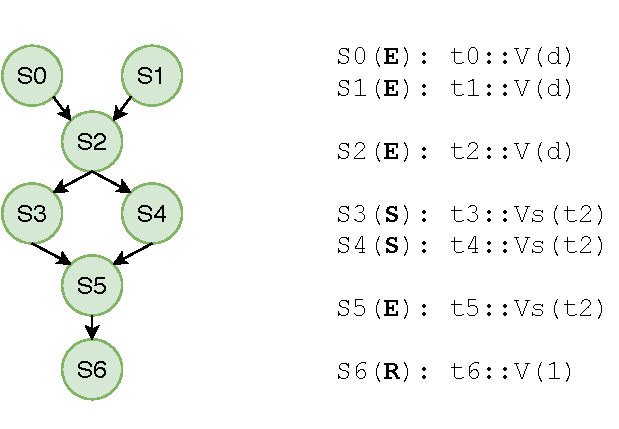
\includegraphics[width=.7\columnwidth]{./src/figure/graph-example.pdf}
\caption{A fusible section for the HorseIR program in \refFig{fig:motivation_horseir}. The
text format on the right hand side is \texttt{<statement>(<group>): <variable>::<shape>}.}
\label{fig:fusion_example}
\end{figure}

Given the HorseIR program in \refFig{fig:motivation_horseir}, our algorithm identifies a
fusible section shown in \refFig{fig:fusion_example}. Initially, the variable \texttt{c0}
is assigned a dynamic vector shape with unique ID, \texttt{V(d)}, as the exact size depends
on the input table. Next, the 3 element-wise functions in statements \texttt{S0},
\texttt{S1}, and \texttt{S2} propagate the vector shape \texttt{V(d)} according to the shape
rules. Both compression functions in \texttt{S3} and \texttt{S4} generate a new shared scan shape
\texttt{Vs(t2)} as they both use the same boolean mask. The following binary function
uses this equality to correctly infer its output shape. Finally, the reduction function
\texttt{@sum} returns a vector with one element. Note that all functions in the computed
fusible section share the same loop range, \texttt{V(d)}.

The code in \refFig{fig:motivation_c} shows the generated C code for the complete
fusible section. Note the presence of an internal condition for the boolean selection
and the accumulator for the reduction. Details of the code generation strategy for fusible
sections are found in \refSec{Sec:codegen}.

% We mainly focus on how to identify fusible subgraphs and generate efficient code correctly.
%\todo{Add an example with a colored CFG tree to show which sections of the tree can be fused.}
% \subsection{Key Parts of the Analysis}

% \hanfeng{You may need to read its source code to see the complete algorithm.
% Sorry for the inconvenience.  It will be changed to a nice format with the latex
% algorithm package later.}



%%% Translated to an algorithm version
%% \begin{lstlisting}[mathescape=true, float=htbp, frame=single]
%% entry:
%%     id $\gets$ 1
%%     depth $\gets$ 0
%%     map $\gets$  $\varnothing$
%%     foreach node A in reversed topological order{
%%         if( !isVisited(A) ) {
%%             if ( A's op is a Reduction ){
%%                 section $\gets$ findFromReduction(A)
%%             }
%%             else {
%%                 section $\gets$ findFusibleSection(A,id)
%%             }
%%             if section is not an empty list
%%                 id $\gets$ id + 1
%%         }
%%     }
%% 
%%     function findFusibleSection(A, id){
%%         setVisited(A)
%%         isFusible = isOpInGroupWithoutR(A)
%%         if(isFusible){
%%             foreach node B in defStmts(A){
%%                 if( B has one use )
%%                     return  {A} $\cup$ findFusibleSection(A, id)
%%                 else{
%%                     if( B is not in map ){
%%                         list $\gets$ findFusibleSection(B, id)
%%                         insert the pair (B, list) into the map
%%                     }
%%                     else list $\gets$ map.get(B)
%%                     return {A} $\cup$ list
%%                 }
%%             }
%%         }
%%         return an empty set
%%     }
%% 
%%     function findFromReduction(A,id){
%%         setVisited(A)
%%         if (size of defStmts(A) is 1){
%%             return {A} $\cup$ findFusibleSection(getDefStmt(A,id))
%%         }
%%         else return {A}
%%     }
%% \end{lstlisting}



%\subsection{Conformable Operations in Groups} \label{SubSec:groups}

% Before generating C code correctly, we need shape rules defined in
% \refTab{table:example_elementwise} for elementwise functions.
% All cases can be determined statically except when both sides are vectors and a
% check for the both sizes is required.

% A set of well-defined primitive functions can be classified into groups
% because of their similar behaviours.  In HorseIR, a function has a fixed
% number of arguments, however, it is allowed to process arguments with
% different shapes.  For instance, \refTable{example:mul} shows the shape rules
% of the multiplication function, \texttt{mul}, having the two arguments which
% can be either a scalar or a vector.

% TODO: show the number of functions in groups 

% \todo{Replace the whole section by using more precise shape abstractions defined before.}

% \todo{Add description for vectors and lists.}

% It should be noted that the loop size is equal to the length of the boolean
% vector so that the condition vector can fit the entire loop correctly.  If two
% shapes with different condition aliases, they have to be conservatively
% considered as different shapes so that a failed shape is returned.
% Therefore, there are several kinds of results after the shape rules:

% \begin{itemize}
% \item \textbf{normal shape} for constant, symbolic, and selection sizes;
% \item \textbf{not conformable but continue} (NCC) for the failure of the shape propagation, but a new symbolic shape is assigned;
% \item \textbf{not conformable and abort} (NCA) for the failure of the shape propagation and the analysis aborts;
% \end{itemize}

% TODO: Type rules for each functions

% \todo{Algorithms for shape propagation.}
